\section*{Circuito}

Il due circuiti che abbiamo utilizzato per questa esperienza sono i seguenti:

\begin{figure}[h]
  \centering
  \begin{subfigure}[b]{0.45\textwidth}
    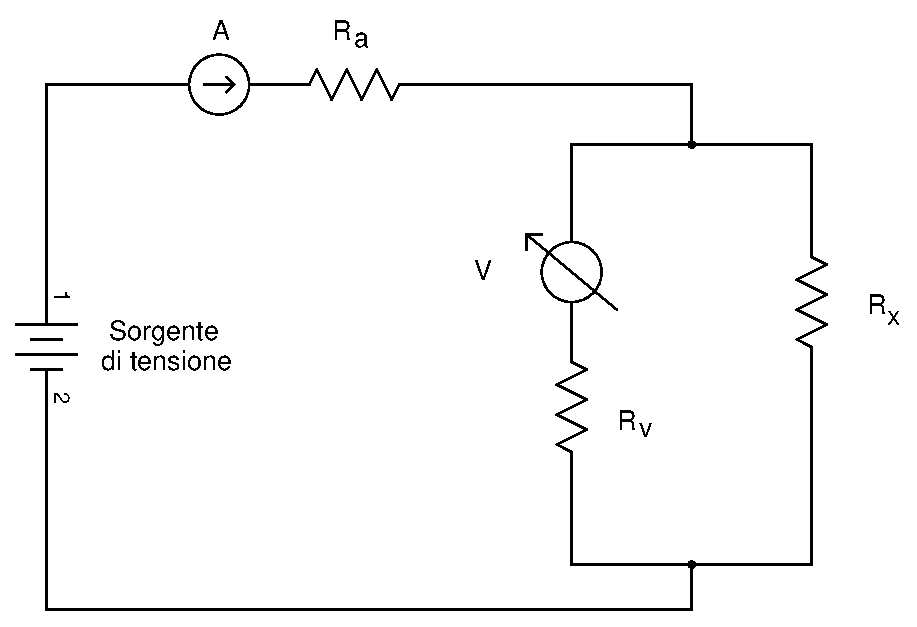
\includegraphics[width=8cm]{monte.eps}
    \caption{Circuito con amperometro a monte}
    \label{fig:monte}
  \end{subfigure}
  \qquad
  \begin{subfigure}[b]{0.45\textwidth}
    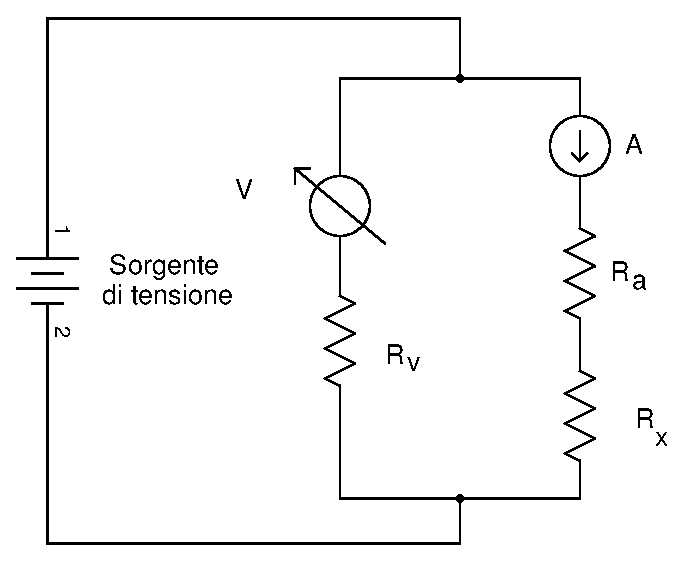
\includegraphics[width=8cm]{valle.eps}
    \caption{Ampetometro a valle}
    \label{fig:valle}
  \end{subfigure}
\end{figure}

Il primo circuito è un circuito con l'amperometro a monte, mentre il secondo circuito è detto circuito con l'amperometro a valle.
Facciamo notare che per impostare la tensione di alimentazione del circuito bisogna fare attenzione a non eccedere la potenza sopportata dalle resistenze analizzate. Il valore di potenza si ricava banalmente sfruttando la legge integrale di Ohm che dice:

\begin{equation}
	V \,=\, \sqrt{W\,R}
\end{equation}

dove $V$ indica la tensione del circuito, $W$ la potenza massima sopportata dalla resistenza e $R$ la resistenza in esame.




